\documentclass[a4paper,14pt]{extreport} % формат документа

\usepackage{amsmath}
\usepackage{cmap} % поиск в ПДФ
\usepackage[T2A]{fontenc} % кодировка
\usepackage[utf8]{inputenc} % кодировка исходного текста
\usepackage[english,russian]{babel} % локализация и переносы
\usepackage[left = 2cm, right = 1cm, top = 2cm, bottom = 2 cm]{geometry} % поля
\usepackage{listings}
\usepackage{graphicx} % для вставки рисунков
\usepackage{amsmath}
\usepackage{float}
\usepackage{multirow}
\graphicspath{{images/}}
\DeclareGraphicsExtensions{.pdf,.png,.jpg}
\newcommand{\anonsection}[1]{\section*{#1}\addcontentsline{toc}{section}{#1}}

\lstset{ %
	language=C,                % Язык программирования 
	numbers=left,                   % С какой стороны нумеровать          
	frame=single,                    % Добавить рамку
	basicstyle=\small,
    escapebegin=\begin{russian}\commentfont,
    escapeend=\end{russian},
    literate={Ö}{{\"O}}1
    {Ä}{{\"A}}1
    {Ü}{{\"U}}1
    {ß}{{\ss}}1
    {ü}{{\"u}}1
    {ä}{{\"a}}1
    {ö}{{\"o}}1
    {~}{{\textasciitilde}}1
    {а}{{\selectfont\char224}}1
    {б}{{\selectfont\char225}}1
    {в}{{\selectfont\char226}}1
    {г}{{\selectfont\char227}}1
    {д}{{\selectfont\char228}}1
    {е}{{\selectfont\char229}}1
    {ё}{{\"e}}1
    {ж}{{\selectfont\char230}}1
    {з}{{\selectfont\char231}}1
    {и}{{\selectfont\char232}}1
    {й}{{\selectfont\char233}}1
    {к}{{\selectfont\char234}}1
    {л}{{\selectfont\char235}}1
    {м}{{\selectfont\char236}}1
    {н}{{\selectfont\char237}}1
    {о}{{\selectfont\char238}}1
    {п}{{\selectfont\char239}}1
    {р}{{\selectfont\char240}}1
    {с}{{\selectfont\char241}}1
    {т}{{\selectfont\char242}}1
    {у}{{\selectfont\char243}}1
    {ф}{{\selectfont\char244}}1
    {х}{{\selectfont\char245}}1
    {ц}{{\selectfont\char246}}1
    {ч}{{\selectfont\char247}}1
    {ш}{{\selectfont\char248}}1
    {щ}{{\selectfont\char249}}1
    {ъ}{{\selectfont\char250}}1
    {ы}{{\selectfont\char251}}1
    {ь}{{\selectfont\char252}}1
    {э}{{\selectfont\char253}}1
    {ю}{{\selectfont\char254}}1
    {я}{{\selectfont\char255}}1
    {А}{{\selectfont\char192}}1
    {Б}{{\selectfont\char193}}1
    {В}{{\selectfont\char194}}1
    {Г}{{\selectfont\char195}}1
    {Д}{{\selectfont\char196}}1
    {Е}{{\selectfont\char197}}1
    {Ё}{{\"E}}1
    {Ж}{{\selectfont\char198}}1
    {З}{{\selectfont\char199}}1
    {И}{{\selectfont\char200}}1
    {Й}{{\selectfont\char201}}1
    {К}{{\selectfont\char202}}1
    {Л}{{\selectfont\char203}}1
    {М}{{\selectfont\char204}}1
    {Н}{{\selectfont\char205}}1
    {О}{{\selectfont\char206}}1
    {П}{{\selectfont\char207}}1
    {Р}{{\selectfont\char208}}1
    {С}{{\selectfont\char209}}1
    {Т}{{\selectfont\char210}}1
    {У}{{\selectfont\char211}}1
    {Ф}{{\selectfont\char212}}1
    {Х}{{\selectfont\char213}}1
    {Ц}{{\selectfont\char214}}1
    {Ч}{{\selectfont\char215}}1
    {Ш}{{\selectfont\char216}}1
    {Щ}{{\selectfont\char217}}1
    {Ъ}{{\selectfont\char218}}1
    {Ы}{{\selectfont\char219}}1
    {Ь}{{\selectfont\char220}}1
    {Э}{{\selectfont\char221}}1
    {Ю}{{\selectfont\char222}}1
    {Я}{{\selectfont\char223}}1
    {і}{{\selectfont\char105}}1
    {ї}{{\selectfont\char168}}1
    {є}{{\selectfont\char185}}1
    {ґ}{{\selectfont\char160}}1
    {І}{{\selectfont\char73}}1
    {Ї}{{\selectfont\char136}}1
    {Є}{{\selectfont\char153}}1
    {Ґ}{{\selectfont\char128}}1
}

\begin{document}
\begin{titlepage}

    \begin{table}[H]
        \centering
        \footnotesize
        \begin{tabular}{cc}
            \multirow{8}{*}{
\includegraphics[scale=0.35]{bmstu}}
            & \\
            & \\
            & \textbf{Министерство науки и высшего образования Российской Федерации} \\
            & \textbf{Федеральное государственное бюджетное образовательное учреждение} \\
            & \textbf{высшего образования} \\
            & \textbf{<<Московский государственный технический} \\
            & \textbf{университет имени Н.Э. Баумана>>} \\
            & \textbf{(МГТУ им. Н.Э. Баумана)} \\
        \end{tabular}
    \end{table}

    \vspace{-2.5cm}

    \begin{flushleft}
        \rule[-1cm]{\textwidth}{3pt}
        \rule{\textwidth}{1pt}
    \end{flushleft}

    \begin{flushleft}
        \small
        ФАКУЛЬТЕТ
        \underline{<<Информатика и системы управления>>\ \ \ \ \ \ \ 
        \ \ \ \ \ \ \ \ \ \ \ \ \ \ \ \ \ \ \ \ \ \ \ \ \ \ \ \ \ \ \ 
    \ \ \ \ \ \ \ \ \ \ \ \ \ \ \ } \\
        КАФЕДРА
        \underline{<<Программное обеспечение ЭВМ и
        информационные технологии>>
        \ \ \ \ \ \ \ \ \ \ \ \ \ \ \ \ \ \ \ \ }
    \end{flushleft}

    \vspace{2cm}

    \begin{center}
        \textbf{Лабораторная работа № 9} \\
        \vspace{0.5cm}
    \end{center}

    \vspace{4cm}

    \begin{flushleft}
        \begin{tabular}{ll}
            \textbf{Дисциплина} & Операционные системы.  \\
            \textbf{Тема} & Обработчики прерываний.  \\
            \\
            \textbf{Студент} & Сиденко А.Г. \\
            \textbf{Группа} & ИУ7-63Б \\
            \textbf{Оценка (баллы)} & \\
            \textbf{Преподаватель} & Рязанова Н.Ю.   \\
        \end{tabular}
    \end{flushleft}

    \vspace{4cm}

   \begin{center}
        Москва, 2020 г.
    \end{center}

\end{titlepage}

\hfill

\textbf{Тасклеты}

\begin{lstlisting}
#include <linux/kernel.h>
#include <linux/module.h>
#include <linux/interrupt.h>
#include <linux/time.h>

MODULE_LICENSE("GPL");
MODULE_AUTHOR("Sidenko");
MODULE_DESCRIPTION("Lab9");

#define MOUSEIRQ 12

char my_tasklet_data[] = "MOUSE IRQ";

// Bottom Half Function
void my_tasklet_function(unsigned long data)
{
  struct timeval t;
  struct tm broken;
  do_gettimeofday(&t);
  time_to_tm(t.tv_sec, 0, &broken);
  printk("%s in: %dd.%dm.%dy %dh:%dm:%ds\n", (char *)data,
			broken.tm_mday, broken.tm_mon + 1,
			broken.tm_year + 1900, broken.tm_hour + 3,
			broken.tm_min, broken.tm_sec);
}

// Регистрация тасклета
DECLARE_TASKLET(my_tasklet, my_tasklet_function, (unsigned long)
						&my_tasklet_data);

// Обработчик прерывания
irqreturn_t irq_handler(int irq, void *dev, struct pt_regs *regs)
{
  // Проверка, что произошло именно нужное 12-е прерывание
  if(irq == MOUSEIRQ)
  {
    // Постановка тасклета в очередь на выполнение
    tasklet_schedule(&my_tasklet);
    return IRQ_HANDLED; // прерывание обработано
  }
  else
    return IRQ_NONE; // прерывание не обработано
}

// Инициализация модуля
static int __init my_module_init(void)
{
  printk(KERN_DEBUG "MODULE loaded!\n");
  // Разделение(совместное использование) линии IRQ с другими устройствами
  int ret = request_irq(MOUSEIRQ, (irq_handler_t)irq_handler, IRQF_SHARED,
				"my_irq_handler", (void *)(irq_handler));
  if (ret != 0)
  {
    printk(KERN_ERR "MOUSE IRQ handler wasn't registered");
    return ret;
  }
  printk(KERN_INFO "MOUSE IRQ handler was registered successfully");
  return ret;
}

// Выход загружаемого модуля
static void __exit my_module_exit(void)
{
  // Освобождение линии прерывания
  free_irq(MOUSEIRQ, (void *)(irq_handler));
  // Удаление тасклета
  tasklet_disable(&my_tasklet);
  tasklet_kill(&my_tasklet);
  printk(KERN_DEBUG "MODULE unloaded!\n");
}

module_init(my_module_init);
module_exit(my_module_exit);
\end{lstlisting}

\begin{enumerate}
\item Загрузим модуль ядра и проверим в списке загруженных модулей ядра

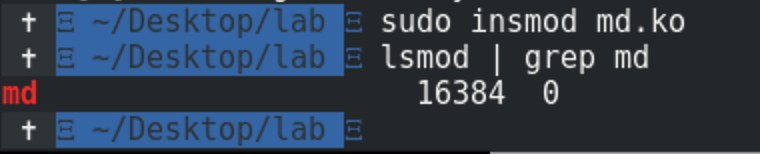
\includegraphics[scale=0.8]{1}

\item Вывод буфера сообщений ядра в стандартный поток вывода

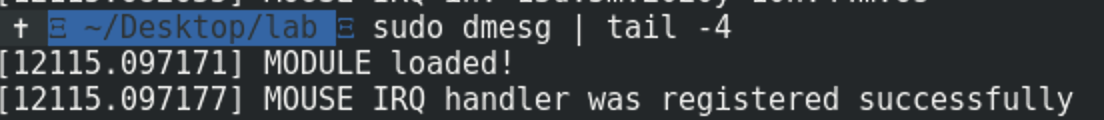
\includegraphics[scale=0.8]{2}

\item Посмотрим содержимое файла /proc/interrupts, который предоставляет таблицу о количестве прерываний на каждом из процессоров

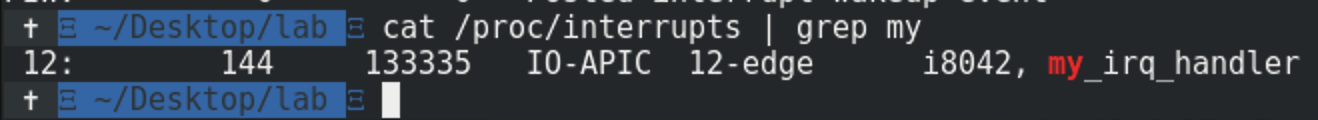
\includegraphics[scale=0.5]{3}

\item Вывод буфера сообщений ядра в стандартный поток вывода, смотрим на обработку прерываний от мыши

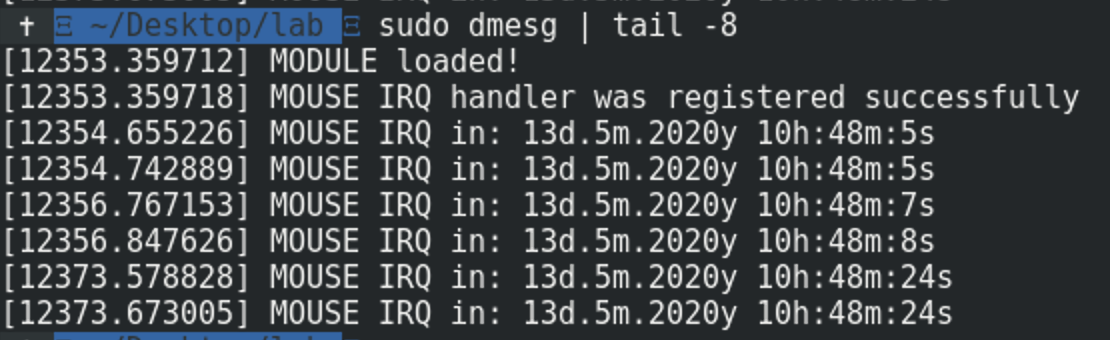
\includegraphics[scale=0.8]{4}

\item Выгружаем модуль ядра и выводим буфер сообщений ядра

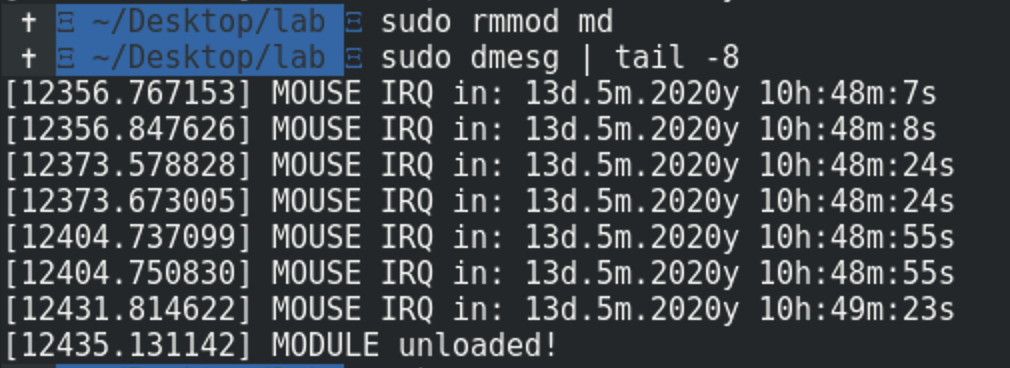
\includegraphics[scale=0.8]{5}

\end{enumerate}

\textbf{Очереди работ}

\begin{lstlisting}
#include <linux/kernel.h>
#include <linux/module.h>
#include <linux/interrupt.h>
#include <linux/time.h>
#include <linux/workqueue.h>
#include <linux/slab.h>

MODULE_LICENSE("GPL");
MODULE_AUTHOR("Sidenko");
MODULE_DESCRIPTION("Lab9");

#define MOUSEIRQ 12

char my_workqueue_data[] = "MOUSE IRQ";
// Очередь работ
static struct workqueue_struct *my_wq;
struct work_struct *my_work;

// Bottom Half Function
void my_workqueue_function(struct work_struct *my_work)
{
  struct timeval t;
  struct tm broken;
  do_gettimeofday(&t);
  time_to_tm(t.tv_sec, 0, &broken);
  printk("%s in: %dd.%dm.%dy %dh:%dm:%ds\n", (char *)my_workqueue_data,
			broken.tm_mday, broken.tm_mon + 1,
			broken.tm_year + 1900, broken.tm_hour + 3,
			broken.tm_min, broken.tm_sec);
  kfree(my_work);
}

irqreturn_t irq_handler(int irq, void *dev, struct pt_regs *regs)
{
  // Проверка, что произошло именно нужное 12-е прерывание
  if(irq == MOUSEIRQ)
  {
    my_work = (struct work_struct*)kmalloc(sizeof(struct work_struct), 
    							GFP_KERNEL);
    if (my_work)	
    {
       INIT_WORK(my_work, my_workqueue_function);
       queue_work(my_wq, my_work);
    }

    return IRQ_HANDLED; // прерывание обработано
  }
  else
    return IRQ_NONE; // прерывание не обработано
}

// Инициализация модуля
static int __init my_module_init(void)
{
  printk(KERN_DEBUG "MODULE loaded!\n");
  // Разделение(совместное использование) линии IRQ с другими устройствами
  int ret = request_irq(MOUSEIRQ, (irq_handler_t)irq_handler, IRQF_SHARED,
				"my_irq_handler", (void *)(irq_handler));
  if (ret != 0)
  {
    printk(KERN_ERR "Mouse IRQ handler wasn't registered");
    return -ENOMEM;
  }

  // Cоздание очереди работ
  my_wq = create_workqueue("my_queue");
  if (my_wq)
    printk(KERN_INFO "Workqueue was allocated successfully");
  else
  {
    free_irq(MOUSEIRQ, (void *)(irq_handler));
    printk(KERN_ERR "Workqueue wasn't allocated");
    return -ENOMEM;
  }

  printk(KERN_INFO "Mouse IRQ handler was registered successfully");
  return ret;
}

// Выход загружаемого модуля
static void __exit my_module_exit(void)
{
  // Освобождение линии прерывания
  free_irq(MOUSEIRQ, (void *)(irq_handler));
  // Удаление очереди работ
  flush_workqueue(my_wq);
  destroy_workqueue(my_wq);
  printk(KERN_DEBUG "MODULE unloaded!\n");
}

module_init(my_module_init);
module_exit(my_module_exit);
\end{lstlisting}

\begin{enumerate}
\item Загрузим модуль ядра и проверим в списке загруженных модулей ядра

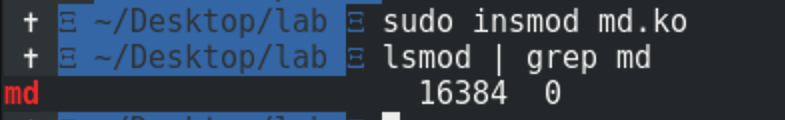
\includegraphics[scale=0.8]{6}

\item Вывод буфера сообщений ядра в стандартный поток вывода

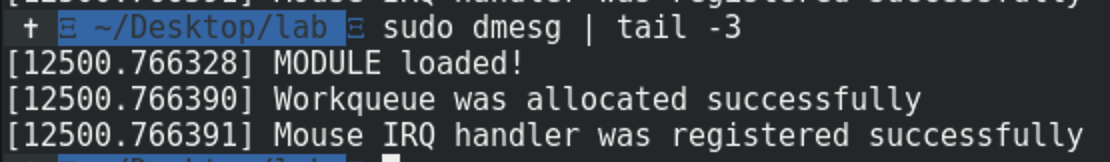
\includegraphics[scale=0.8]{7}

\item Посмотрим содержимое файла /proc/interrupts, который предоставляет таблицу о количестве прерываний на каждом из процессоров

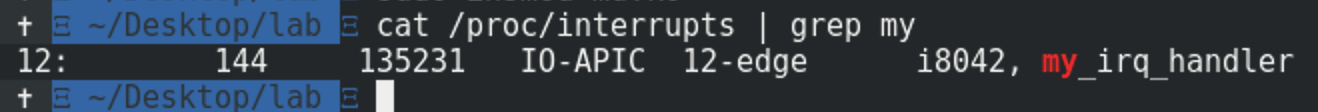
\includegraphics[scale=0.5]{8}

\item Вывод буфера сообщений ядра в стандартный поток вывода, смотрим на обработку прерываний от мыши

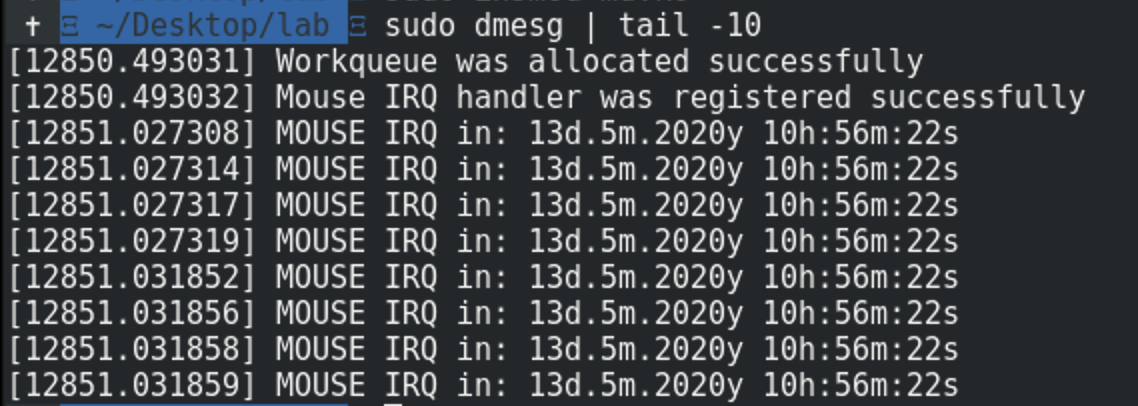
\includegraphics[scale=0.8]{9}

\item Выгружаем модуль ядра и выводим буфер сообщений ядра

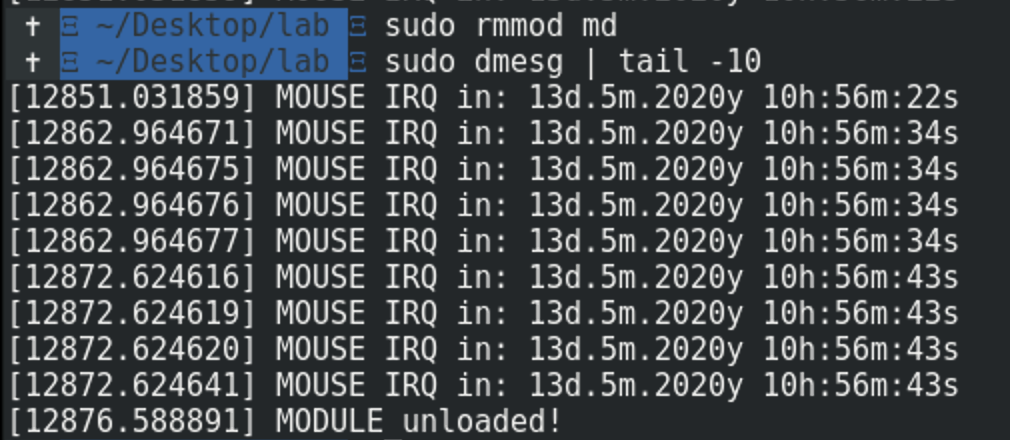
\includegraphics[scale=0.8]{10}

\end{enumerate}

\textbf{Makefile}

\begin{lstlisting}
ifneq ($(KERNELRELEASE),)
	obj-m := md.o
else
	CURRENT = $(shell uname -r)
	KDIR = /lib/modules/$(CURRENT)/build
	PWD = $(shell pwd)

default:
	$(MAKE) -C $(KDIR) M=$(PWD) modules

clean:
	rm -rf .tmp_versions
	rm *.ko
	rm *.o
	rm *.mod.c
	rm *.symvers
	rm *.order

endif
\end{lstlisting}

\end{document}